\documentclass{standalone}
\usepackage{tikz}
\usepackage{xcolor}
\usetikzlibrary{patterns, positioning}
\usetikzlibrary{shapes.misc}
\usepackage[outline]{contour}
\contourlength{1.5pt} 


\begin{document}
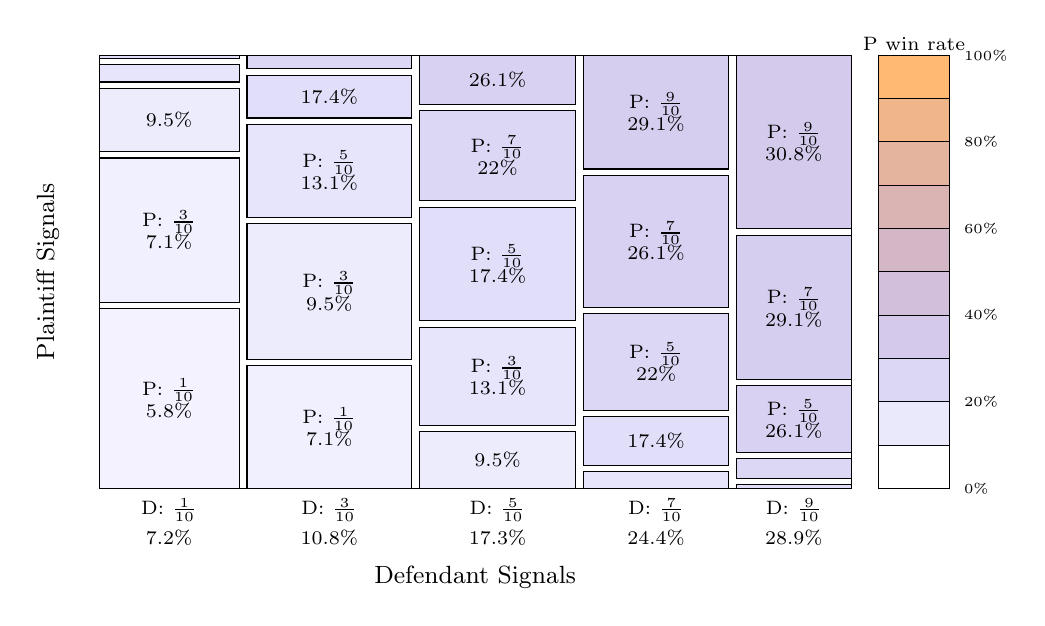
\begin{tikzpicture}
\newcommand{\DFractionOffset}{0.4}
\newcommand{\AxisLabelYAdjust}{-0.235}
\draw[draw=black] (0.6,2) rectangle (10.15,7.5);
\draw[fill=blue!94!orange!6!white!86!white, draw=black] (0.6,2) rectangle (2.3783,4.2797);
\draw (1.4891380319810916, 3.1398563685502645) node[font=\scriptsize, text=black, align=center] {P: $\frac{1}{10}$\\ 5.8\%};
\draw[fill=blue!93!orange!7!white!86!white, draw=black] (0.6,4.3597) rectangle (2.3783,6.1961);
\draw (1.4891380319810916, 5.277925889975353) node[font=\scriptsize, text=black, align=center] {P: $\frac{3}{10}$\\ 7.1\%};
\draw[fill=blue!91!orange!9!white!85!white, draw=black] (0.6,6.2761) rectangle (2.3783,7.081);
\draw (1.4891380319810916, 6.678560264961166) node[font=\scriptsize, text=black, align=center] {9.5\%};
\draw[fill=blue!87!orange!13!white!84!white, draw=black] (0.6,7.161) rectangle (2.3783,7.38);
\draw[fill=blue!83!orange!17!white!82!white, draw=black] (0.6,7.46) rectangle (2.3783,7.5);
\draw (1.4891380319810916, 1.6) node[anchor=north, font=\scriptsize, text=black] {7.2\%};
\draw (1.4891380319810916, {1.6 + \DFractionOffset}) node[anchor=north, font=\scriptsize, text=black] {D: $\frac{1}{10}$};
\draw[fill=blue!93!orange!7!white!86!white, draw=black] (2.4783,2) rectangle (4.5688,3.5621);
\draw (3.523544153532146, 2.7810610922047374) node[font=\scriptsize, text=black, align=center] {P: $\frac{1}{10}$\\ 7.1\%};
\draw[fill=blue!91!orange!9!white!85!white, draw=black] (2.4783,3.6421) rectangle (4.5688,5.3635);
\draw (3.523544153532146, 4.50279658382897) node[font=\scriptsize, text=black, align=center] {P: $\frac{3}{10}$\\ 9.5\%};
\draw[fill=blue!87!orange!13!white!84!white, draw=black] (2.4783,5.4435) rectangle (4.5688,6.6238);
\draw (3.523544153532146, 6.033622857746502) node[font=\scriptsize, text=black, align=center] {P: $\frac{5}{10}$\\ 13.1\%};
\draw[fill=blue!83!orange!17!white!82!white, draw=black] (2.4783,6.7038) rectangle (4.5688,7.2481);
\draw (3.523544153532146, 6.97591269135981) node[font=\scriptsize, text=black, align=center] {17.4\%};
\draw[fill=blue!78!orange!22!white!81!white, draw=black] (2.4783,7.3281) rectangle (4.5688,7.5);
\draw (3.523544153532146, 1.6) node[anchor=north, font=\scriptsize, text=black] {10.8\%};
\draw (3.523544153532146, {1.6 + \DFractionOffset}) node[anchor=north, font=\scriptsize, text=black] {D: $\frac{3}{10}$};
\draw[fill=blue!91!orange!9!white!85!white, draw=black] (4.6688,2) rectangle (6.6509,2.7221);
\draw (5.659851997385145, 2.361043047878584) node[font=\scriptsize, text=black, align=center] {9.5\%};
\draw[fill=blue!87!orange!13!white!84!white, draw=black] (4.6688,2.8021) rectangle (6.6509,4.047);
\draw (5.659851997385145, 3.424530270924455) node[font=\scriptsize, text=black, align=center] {P: $\frac{3}{10}$\\ 13.1\%};
\draw[fill=blue!83!orange!17!white!82!white, draw=black] (4.6688,4.127) rectangle (6.6509,5.5707);
\draw (5.659851997385145, 4.8488246249885165) node[font=\scriptsize, text=black, align=center] {P: $\frac{5}{10}$\\ 17.4\%};
\draw[fill=blue!78!orange!22!white!81!white, draw=black] (4.6688,5.6507) rectangle (6.6509,6.7995);
\draw (5.659851997385145, 6.225084983994322) node[font=\scriptsize, text=black, align=center] {P: $\frac{7}{10}$\\ 22\%};
\draw[fill=blue!74!orange!26!white!79!white, draw=black] (4.6688,6.8795) rectangle (6.6509,7.5);
\draw (5.659851997385145, 7.189747582051677) node[font=\scriptsize, text=black, align=center] {26.1\%};
\draw (5.659851997385145, 1.6) node[anchor=north, font=\scriptsize, text=black] {17.3\%};
\draw (5.659851997385145, {1.6 + \DFractionOffset}) node[anchor=north, font=\scriptsize, text=black] {D: $\frac{5}{10}$};
\draw[fill=blue!87!orange!13!white!84!white, draw=black] (6.7509,2) rectangle (8.5965,2.211);
\draw[fill=blue!83!orange!17!white!82!white, draw=black] (6.7509,2.291) rectangle (8.5965,2.9075);
\draw (7.67371887569091, 2.59928824844115) node[font=\scriptsize, text=black, align=center] {17.4\%};
\draw[fill=blue!78!orange!22!white!81!white, draw=black] (6.7509,2.9875) rectangle (8.5965,4.2213);
\draw (7.67371887569091, 3.6044024178809604) node[font=\scriptsize, text=black, align=center] {P: $\frac{5}{10}$\\ 22\%};
\draw[fill=blue!74!orange!26!white!79!white, draw=black] (6.7509,4.3013) rectangle (8.5965,5.9767);
\draw (7.67371887569091, 5.139007795190618) node[font=\scriptsize, text=black, align=center] {P: $\frac{7}{10}$\\ 26.1\%};
\draw[fill=blue!71!orange!29!white!78!white, draw=black] (6.7509,6.0567) rectangle (8.5965,7.5);
\draw (7.67371887569091, 6.778372152034858) node[font=\scriptsize, text=black, align=center] {P: $\frac{9}{10}$\\ 29.1\%};
\draw (7.67371887569091, 1.6) node[anchor=north, font=\scriptsize, text=black] {24.4\%};
\draw (7.67371887569091, {1.6 + \DFractionOffset}) node[anchor=north, font=\scriptsize, text=black] {D: $\frac{7}{10}$};
\draw[fill=blue!83!orange!17!white!82!white, draw=black] (8.6965,2) rectangle (10.15,2.0489);
\draw[fill=blue!78!orange!22!white!81!white, draw=black] (8.6965,2.1289) rectangle (10.15,2.3762);
\draw[fill=blue!74!orange!26!white!79!white, draw=black] (8.6965,2.4562) rectangle (10.15,3.3024);
\draw (9.42327299985682, 2.879324729416155) node[font=\scriptsize, text=black, align=center] {P: $\frac{5}{10}$\\ 26.1\%};
\draw[fill=blue!71!orange!29!white!78!white, draw=black] (8.6965,3.3824) rectangle (10.15,5.2151);
\draw (9.42327299985682, 4.2987688830114195) node[font=\scriptsize, text=black, align=center] {P: $\frac{7}{10}$\\ 29.1\%};
\draw[fill=blue!69!orange!31!white!78!white, draw=black] (8.6965,5.2951) rectangle (10.15,7.5);
\draw (9.42327299985682, 6.397560449429717) node[font=\scriptsize, text=black, align=center] {P: $\frac{9}{10}$\\ 30.8\%};
\draw (9.42327299985682, 1.6) node[anchor=north, font=\scriptsize, text=black] {28.9\%};
\draw (9.42327299985682, {1.6 + \DFractionOffset}) node[anchor=north, font=\scriptsize, text=black] {D: $\frac{9}{10}$};
\node[font=\small, text=black] at (5.375, {1.1 + \AxisLabelYAdjust}) {Defendant Signals};
\node[font=\small, text=black, rotate=90] at (-0.050000000000000044, 4.75) {Plaintiff Signals};
\draw[draw=black] (10.5,2) rectangle (11.4,7.5);
\draw (10.95, 7.65) node[font=\scriptsize, text=black] {P win rate};
\draw[fill=blue!100!orange!0!white!88!white, draw=black] (10.5,2) rectangle (11.4,2.55);
\draw[fill=blue!89!orange!11!white!84!white, draw=black] (10.5,2.55) rectangle (11.4,3.1);
\draw[fill=blue!78!orange!22!white!81!white, draw=black] (10.5,3.1) rectangle (11.4,3.65);
\draw[fill=blue!67!orange!33!white!77!white, draw=black] (10.5,3.65) rectangle (11.4,4.2);
\draw[fill=blue!56!orange!44!white!73!white, draw=black] (10.5,4.2) rectangle (11.4,4.75);
\draw[fill=blue!44!orange!56!white!70!white, draw=black] (10.5,4.75) rectangle (11.4,5.3);
\draw[fill=blue!33!orange!67!white!66!white, draw=black] (10.5,5.3) rectangle (11.4,5.85);
\draw[fill=blue!22!orange!78!white!62!white, draw=black] (10.5,5.85) rectangle (11.4,6.4);
\draw[fill=blue!11!orange!89!white!59!white, draw=black] (10.5,6.4) rectangle (11.4,6.95);
\draw[fill=blue!0!orange!100!white!55!white, draw=black] (10.5,6.95) rectangle (11.4,7.5);
\draw (11.46, 2) node[anchor=west, font=\tiny, text=black] {0\%};
\draw (11.46, 3.1) node[anchor=west, font=\tiny, text=black] {20\%};
\draw (11.46, 4.2) node[anchor=west, font=\tiny, text=black] {40\%};
\draw (11.46, 5.3) node[anchor=west, font=\tiny, text=black] {60\%};
\draw (11.46, 6.4) node[anchor=west, font=\tiny, text=black] {80\%};
\draw (11.46, 7.5) node[anchor=west, font=\tiny, text=black] {100\%};


\end{tikzpicture}
\end{document}